\chapter{Background and Related work}
\label{chap:background}

\section{Web page structure}
Every day we face various webpages through the computer or mobile phone. Few of us realize what processes and intermediate steps behind the webpage which the browser displays us. In the Internet a webpage retrieves the information from the remote web server by sending HTTP requests. We won't discuss the process of requesting, rather we will explain the intermediate steps between the stage when the browser retrieved the information from the server and displays it to the user. \\

A webpage as a set of available information may contain a lot of different information:

\begin{itemize}
    \item Textual information which we see
    \itme Static media files as images, video files, animated GIF, SVG, etc.
    \item Dynamic media as Flash, Java applets, HTML5.
    \item Hyperlinks, buttons and other components which we can interact with.
    \item Semantic meta-information.
    \item JavaScript scripts which add interactivity and additional functionality.
    \item Cascading Style Sheets (CSS) files which say how to rendered the webpage.
\end{itemize}

A webpage may or may not have a specific \textit{Uniform Resource Locator} (URL). Today more and more websites prefer dynamic pages where the same URL addresses can be associated with different pages. It's not convenient for a search engines, that's why they ask for a static pages with unique permalink for the most important pages. \\

\begin{enumerate}
    \item The browser retrieved the HTML and CSS files.
    \item The browser builds the Document Object Model (DOM) tree from a HTML code. The DOM contains the objects which define the structure and content of the page.
    \item The browser builds the CSSOM tree visualization model from CSS files. CSSOM contains the objects which define the style of all elements in DOM.
    \item The DOM and CSSOM trees are combined to form the Render tree. Render tree doesn't include the hidden nodes as script, meta tags, an so on. Also some nodes are hidden because it was reflected in the CSS files (explicit property "display: none").
    \item Render tree contains only the nodes which required to render the page.
    \item The browser is building the layout and computes the exact position and size of each object.
    \item The paint stage is when the browser takes the render tree and render pixels to the screen. 
    
\end{enumerate}


Scheme of how the browser show the page: HTML + CSS -> DOM --> Layout --> Rendering, etc

% \subsubsection{DOM, HTML, CSS, JavaScript}
\section{Web extraction}

The data in the Internet is very massive and heterogeneous. Every website is following it's own design and structure, presenting the same information in a different way for the specific audience of the website. World Wide Web Consortium (W3C) is an international standard organization. tries to get all the players on the Web implement the same set of core principles and components, use the same technologies and standards. 

\begin{figure}[h]
\begin{center}
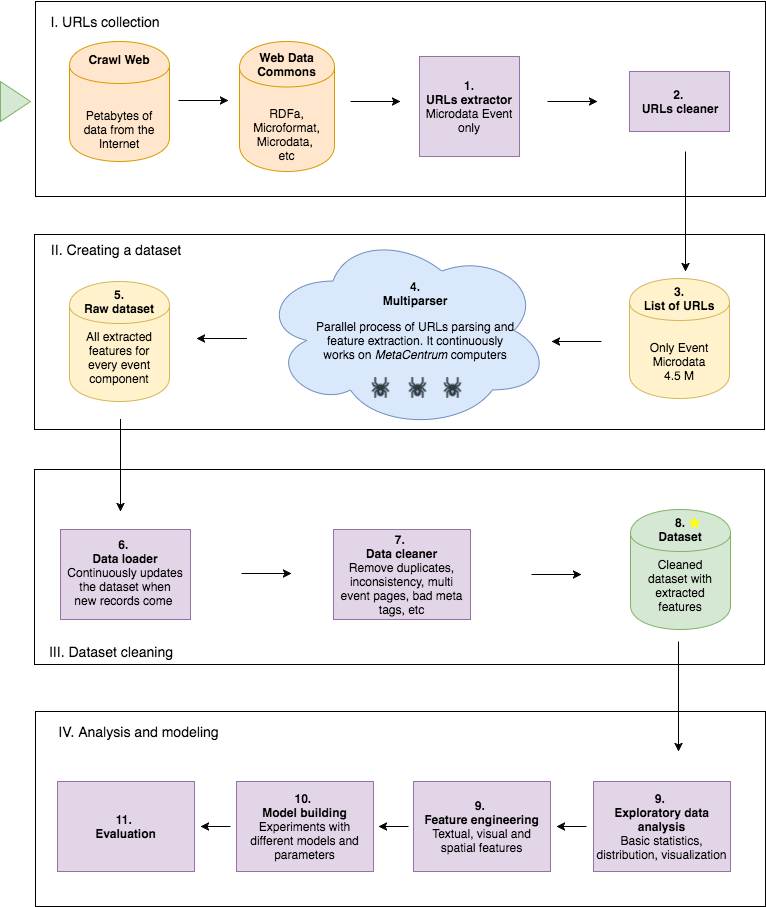
\includegraphics[width=1.0\textwidth]{figures03/Architecure}
\caption{The components of Sociopath event extraction system}
\label{fig:architecture}
\end{center}
\end{figure}


\subsection{Web extraction methods}
\subsubsection{Wrappers}
\subsubsection{Adaptive information extraction}
\subsection{Other related techniques}
\subsubsection{Region extraction}
\subsubsection{Visual segmentation}
\subsection{Recall and Precision}
\subsection{Web extraction as a service}
\section{Semantic web}
\subsection{Microformats, RDF}
\subsection{Semantic web pervasiveness}
\section{Related works}


